\documentclass{article}
\usepackage[utf8]{inputenc}
\usepackage{geometry}
\usepackage{amssymb}
\usepackage{amsmath}
\usepackage{listings}
\usepackage{array}
\usepackage{calc}
\usepackage{graphicx}
\usepackage{subfig}

\usepackage{tikz}

\usepackage{biblatex} %Imports biblatex package
\addbibresource{ref.bib} %Import the bibliography file

\usepackage[linesnumbered]{algorithm2e}
\usepackage{hyperref}
\usepackage{setspace}
\renewcommand*\contentsname{Summary}

\geometry{hmargin=3.5cm,vmargin=1.5cm}

\title{Internship Report}
\author{Solal Rapaport }
\date{June 2022}

\begin{document}

\maketitle
\doublespacing
\tableofcontents
\singlespacing
\newpage

\section{Introduction}

There are two goals here, the first one is to build formulas that will allow robots, spread on a ring, to gather. We have $k$ robots and we will use view vectors to build those formulas. The formulas will be an interpretation of the pseudo-code given in the research report \cite{gathering}.

The formulas we are building, will be used with formulas given in an other research report \cite{algo}, and then will be tested in the acceleration algorithm using an interpolant \cite{algo}. Which leads us to the second goal, we want to implement and, if possible, improve this algorithm.

\section{Logical Formulas}

In this section, we will translate the algorithms given in the research report \cite{gathering}. Some changes will have to be made because we can't literally translate an algorithm into a first-order logic formula.

Before each formula we will describe briefly their scope : when will they be true (or false). We won't present to you the implementation of those formulas in this report. There will be an annex available with the \textit{Python} implementation that we use in order to test those formulas and to put them in the algorithm \cite{algo}.

We have three strategies. Each of them allows a robot to move in a given direction based on its environment. They all have the same definition, they take one argument : the view vector (distance vector).

\subsection{Configurations with single multiplicity}

The strategy $\phi_{SM}$ is $true$ if the given configuration has a single multiplicity and that the robot calling the strategy should move toward the robot at distance $d_{0}$ :
\begin{center}
$\phi_{SM}(d_0, \ldots , d_{k-1}):=$\\
$(\bigvee_{i=0}^{k-1}(d_i = 0\bigwedge_{j=0\ j\not=i}^{k-1} (d_j > 0 \lor (d_j = 0 \land d_{j-1} = 0) ) ))\land$\\
$(d_{k-1} \not= 0) \land $\\
$((d_1 = 0 \land d_{k-2} = 0 \land d_0 \leq d_{k-1}) \lor (d_1 = 0 \land d_{k-2} \not= 0))$
\end{center}

In order to test our strategy we need a function that will initialize our first configuration and make it one with a single multiplicity without being already a winning one, we just thought it'd be a neat thing to do. Here is the formula $InitSM$ which is $true$ if $p$, $s$ and $t$ form a configuration with a single multiplicity, the configuration is not a winning one, all $p$ are initialized in the right scope, all $t$ are initialized at $0$ and all $s$ are initialized at $RLC$ ($-1$) :

\begin{center}
    
$InitSM(p_{0},\dots, p_{k-1}, s_{0}, \dots, s_{k-1}, t_{0}, \dots, t_{k-1}, size_{ring}):=$\\
$\bigvee_{i = 0}^{k-1}( p_{i} \not= p_{i+1 \mod{k-1}} ) \land$\\
$(\bigwedge_{i = 0}^{k-1} ( p_{i} \geq 0 \land p_{i} <  size_{ring} \land s_{i} = -1 \land t_{i} = 0)) \land$\\
$(\bigvee_{i = 0}^{k-1} (\bigvee_{j = 0, j\not=i}^{k-1} (p_{j} = p_{i} \land \bigwedge_{h = 0}^{k-1} ( \bigwedge_{l = 0, l\not=h}^{k-1} (p_{h} \not= p_{l} \lor p_{h} = p_{i}) ) ) ) )$
\end{center}

\begin{figure}[!hp]
    \centering
    \def\svgscale{0.3}
    \input{dessinSM.pdf_tex}
    \caption{Single multiplicity configuration. Here, the view vector or C is (4, 0, 5, 3). Because there's only one 0 we know there is a single multiplicity. Because the 0 isn't the last int of the vector we know C is not on the multiplicity. There's only one free segment toward the multiplicity, hence C can move on this segment.}
    \label{dessinSM}
\end{figure}

\subsection{Gathering rigid configurations}

Let $d_{ij}$ be the value $j$ of the view vector of the robot $i$, and $ds_{ij}$ the value $j$ of the symmetrical 
view of the robot $i$.
The robot is calling the strategy $\phi_R$.

Here are all the logic formulas used in order to build $\phi_R$:\newline


$AllView$ is $true$ if $d_{00}, \ldots ,d_{k-1k-1}$ are all the views you can obtain from a single view vector $dist_{0}, \ldots ,dist_{k-1}$ :

\begin{center}
    
$AllView(dist_{0}, \ldots ,dist_{k-1}, d_{00}, \ldots ,d_{k-1k-1}):=$\\
$(\bigwedge_{i=0}^{k-1} (\bigwedge_{j=0}^{k-1} (d_{ij} = dist_{(j+i) \mod{k}}) ) )$
\end{center}

$IsRigid$ is $true$ if the given configuration is a rigid configuration. Meaning, all views are distinct, there is no multiplicity, and the configuration isn't symmetric nor periodic.

\begin{center}

$IsRigid(d_{00}, \ldots ,d_{k-1k-1}, ds_{00}, \ldots ,ds_{k-1k-1}):=$\\
$\bigwedge_{i=0}^{k-1}(\bigwedge_{j=0}^{k-1}d_{ij}\not=0)\land $\\%pas de multiplicité
$\bigwedge_{i=0}^{k-1}(
\bigwedge_{l=0\ l\not=i}^{k-1}(
(\bigvee_{j=0}^{k-1}d_{ij} \not= d_{lj})
\land (\bigvee_{j=0}^{k-1}d_{ij} \not= ds_{lj})$\\
$\land (\bigvee_{j=0}^{k-1}ds_{ij} \not= d_{lj})
\land (\bigvee_{j=0}^{k-1}ds_{ij} \not= ds_{lj})
) )$\\%Toutes les vues sont distinctes
\end{center}

$AllCode$ is $true$ if $(\alpha'_{r}, \beta'_{r})$ is the set of two natural numbers of the robot $r$ such as $\alpha'_r$ and $\beta'_r$ are codes of $r$'s views, with $\alpha'_{r} < \beta'_{r}$. The process which leads us to obtain all view codes is defined in the research report \cite{gathering}. 

\begin{center}
$AllCode(d_{00}, \ldots ,d_{k-1k-1}, ds_{00}, \ldots ,ds_{k-1k-1}, \alpha_{0}, \dots, \alpha_{k-1}, \beta_{0}, \dots, \beta_{k-1},$\\
$\alpha'_{0}, \dots, \alpha'_{k-1}, \beta'_{0}, \dots, \beta'_{k-1}) :=$\\
$\bigwedge_{i = 0}^{k-1} \left( \alpha'_{i} < \beta'_{i} \land (\alpha'_{i} = \alpha_{i} \lor \alpha'_{i} = \beta_{i}) \land (\beta'_{i} = \alpha_{i} \lor \beta'_{i} = \beta_{i}) \right) \land $\\
$($
$(\alpha_{0} < \alpha_{1} < \dots < \alpha_{k-1} < \beta_{0} < \dots < \beta_{k-1}) \land $\\
$(\bigvee_{p=0}^{k-1}(\bigwedge_{q=0}^{p-1}(d_{0q} = d_{1q}) \land d_{0p} > d_{1p} ) )\land \dots \land $\\
$(\bigvee_{p=0}^{k-1}(\bigwedge_{q=0}^{p-1}(ds_{(k-2)q} = ds_{(k-1)q}) \land ds_{(k-2)p} > ds_{(k-1)p} ) )$\\
$\lor $\\
$((\alpha_{0} < \alpha_{2} < \alpha_{1} < \dots < \alpha_{k-1} < \beta_{0} < \dots < \beta_{k-1}) \land \dots) \lor \dots$
$)$
\end{center}

$CodeMaker$ is $true$ if the configuration is rigid and if $(a_{0}, \ldots , a_{k-1}, as_{0}, \ldots , as_{k-1})$ are each code of each view passed as a parameter :

\begin{center}
$CodeMaker(d_{00}, \ldots ,d_{k-1k-1}, ds_{00}, \ldots ,ds_{k-1k-1}, a_{0}, \ldots , a_{k-1}):=$\\
$IsRigid(d_{00}, \ldots ,d_{k-1k-1}, ds_{00}, \ldots ,ds_{k-1k-1}) \land $\\
%   le couple (alpha', beta') le premier ordre lexicographique, couple d'entier ordonné
%   alpha code vue, beta code de vue symétrique
$\exists \alpha_{0}, \dots, \alpha_{k-1}, \beta_{0}, \dots, \beta_{k-1},$
$\alpha'_{0}, \dots, \alpha'_{k-1}, \beta'_{0}, \dots, \beta'_{k-1},$\\
$AllCode(d_{00}, \ldots ,d_{k-1k-1}, ds_{00}, \ldots ,ds_{k-1k-1}, \alpha_{0}, \dots, \alpha_{k-1}, \beta_{0}, \dots, \beta_{k-1}, $\\
$\alpha'_{0}, \dots, \alpha'_{k-1}, \beta'_{0}, \dots, \beta'_{k-1})$\\
$(\bigwedge_{i = 0}^{k-1} (\bigwedge_{j = 0, j\not=i}^{k-1} ((a_{i} > a_{j} \land \alpha'_{j} > \alpha'_{i}) \lor (a_{i} < a_{j} \land \alpha'_{j} < \alpha'_{i}) ) ) )$\\
$\bigwedge_{i=0}^{k-1} (\bigwedge_{j=0, j \not= i}^{k-1} a_{i} \not= a_{j})$
\end{center}

$FindMax$ is $true$ if $Max$ is the highest value of the view vector passed as a parameter :

\begin{center}

$FindMax(dist_{0}, \ldots ,dist_{k-1}, Max):=$\\
$(\bigwedge_{i=0}^{k-1} (Max \geq dist_{i}) \land (\bigvee_{i=0}^{k-1} (Max = dist_{i})))$
\end{center}

$FindM$ is $true$ if $M$ is the index of the robot (index in the view vector) which has the largest code of view and a neighboring robot at distance $Max$ :

\begin{center}

$FindM(d_{00}, \ldots ,d_{k-1k-1}, a_{0}, \ldots , a_{k-1}, Max, dM_{0}, \dots, dM_{k-1}):=$\\
$\bigvee_{m=0}^{k-1}((\bigwedge_{i=0}^{k-1} ((a_{m} \geq a_i \land (d_{i0} = Max \lor d_{ik-1} = Max))$\\
$\lor (d_{i0} < Max \land d_{ik-1} < Max))) \land M = m )$
\end{center}

$FindN$ is $true$ if $N$ is the index of the robot (index in the view vector) with the largest code of view and $M$ as a neighboring robot at distance $Max$ :

\begin{center}

$FindN(d_{00}, \ldots ,d_{k-1k-1}, a_{0}, \ldots , a_{k-1}, Max, M, N):=$\\
$(d_{M0} = Max \land d_{Mk-1} = Max \land $\\
$( (N = ((M+1) \mod{k}) \land a_{(M+1) \mod{k}} > a_{(M-1) \mod{k}}) \lor $\\
$(N = ((M-1) \mod{k}) \land a_{(M-1) \mod{k}} > a_{(M+1) \mod{k}})))$\\
$ \lor$\\
$(d_{M0} = Max \land d_{Mk-1} \not= Max \land N = ((M+1)\mod{k}))$\\
$ \lor$\\
$(d_{M0} \not= Max \land d_{Mk-1} = Max \land N = ((M-1)\mod{k}))$
\end{center}

Since those formulas can't be implemented in \textit{Python} because it is impossible to work around a variable index, we choose to build a new formula, $FindMN$ that will be $true$ if both vectors $dM$ and $dN$ are the view vector of, respectively, $M$ and $N$.

\begin{center}

$FindMN(d_{00}, \ldots ,d_{k-1k-1}, a_{0}, \ldots , a_{k-1}, Max, M, N,$\\
$ dM_{0}, \dots, dM_{k-1}, dN_{0}, \dots, dN_{k-1}):=$\\
$\bigvee_{m=0}^{k-1}(\quad
(\bigwedge_{i=0}^{k-1} ((a_{m} \geq a_i \land (d_{i0} = Max \lor d_{ik-1} = Max))$\\
$\lor (d_{i0} < Max \land d_{ik-1} < Max))) \land M = m \land $\\ 
%(\bigwedge_{l = 0}^{k-1} (dM_{l} = d_{ml}) )
%(\bigwedge_{l = 0}^{k - 1} (dN_{l} = d_{(m+1 \mod{k}) l}) )
%(\bigwedge_{l = 0}^{k - 1} (dN_{l} = d_{(m-1 \mod{k}) l}) )
$(\quad (
d_{m0} = Max \land d_{mk-1} = Max \land $\\
$( ( N = M+1 \mod k \land a_{(m+1) \mod{k}} > a_{(m-1) \mod{k}}) \lor $\\
$( N = M-1 \mod{k} \land a_{(m-1) \mod{k}} > a_{(m+1) \mod{k}}))
)\lor $\\
$(
d_{m0} = Max \land d_{mk-1} \not= Max \land N = M+1 \mod k
) \lor$\\
$(
d_{m0} \not= Max \land d_{mk-1} = Max \land N = M-1 \mod{k}
)\quad ) \land $\\
$( (N = M-1\mod{k} \land (\bigwedge_{l = 0}^{k-1} (dN_{l} = d_{(m-1 \mod{k}) ((k-1)-l)} \land dM_{l} = d_{ml}) ) ) \lor $\\
$(N = M+1\mod{k} \land (\bigwedge_{l = 0}^{k-1} (dN_{l} = d_{(m+1 \mod{k})l} \land dM_{l} = d_{m((k-1)-l)}) ) ) )$
$\quad )$
\end{center}

$\phi_R$ is $true$ if the configuration is rigid, and if the robot is $M$ and has a closest neighbor than $N$, or if the robot is $N$ and has a closest neighbor than $M$.

\begin{center}

$\phi_R(dist_{0}, \ldots ,dist_{k-1}):=$\\
$\exists d_{00}, \ldots ,d_{k-1k-1},\ AllView(dist_{0}, \ldots ,dist_{k-1}, d_{00}, \ldots ,d_{k-1k-1})\land$\\
$\exists ds_{00}, \ldots ,ds_{k-1k-1}, \bigwedge_{i=0}^{k-1} (ViewSym(d_{i0}, \ldots , d_{ik-1}, ds_{i0}, \ldots , ds_{ik-1}))\land$\\
$\exists Max, a_{0}, \ldots , a_{k-1}, dM_{0}, \dots, dM_{k-1}, dN_{0}, \dots, dN_{k-1},$\\
%on fait les codes de vues
$CodeMaker(d_{00}, \ldots ,d_{k-1k-1}, ds_{00}, \ldots ,ds_{k-1k-1}, a_{0}, \ldots , a_{k-1})\land$\\
%On initialise Max, M et N
$FindMax(dist_{0}, \ldots ,dist_{k-1}, Max) \land$\\
%Initialiser M et N
$FindMN(d_{00}, \ldots ,d_{k-1k-1}, a_{0}, \ldots , a_{k-1}, Max,  dM_{0}, \dots, dM_{k-1}, dN_{0}, \dots, dN_{k-1}) \land $\\
$\exists dM2_{0}, \dots, dM2_{k-1}, dN2_{0}, \dots, dN2_{k-1},$\\
$( (\bigwedge_{i = 0}^{k-1} (dM2_{i} = dM_{i+1 \mod{k}}) ) \lor (\bigwedge_{i = 0}^{k-1} (dM2_{i} = dM_{i-1 \mod{k}})) ) \land$\\
$(\bigvee_{i = 0}^{k-1} (dM2_{i} \not= dN_{i}) ) \land $\\
$( (\bigwedge_{i = 0}^{k-1} (dN2_{i} = dN_{i+1 \mod{k}}) ) \lor (\bigwedge_{i = 0}^{k-1} (dN2_{i} = dN_{i-1 \mod{k}})) ) \land$\\
$(\bigvee_{i = 0}^{k-1} (dN2_{i} \not= dM_{i}) ) \land $\\

%On initialise toutes les distances possibles par rapport à M et N
$\exists distM_{0}, \ldots , distM_{k-1}, distN_{0}, \ldots , distN_{k-1},$\\
$\bigwedge_{i=0}^{k-1}(distM_{i} = (\sum_{l=0}^i dM_{l}) \land distN_{i} = (\sum_{l=0}^i dN_{l}) ) \land $\\
$(\bigvee_{i=0}^{k-1}\quad (\quad (distM_{i} < distN_{i} \bigwedge_{q=0}^{i} (distM_{q} = distN_{q}) \bigwedge_{j = 0}^{k-1} (dM_{j} = dist_{j}) ) \lor $\\
$(distM_{i} > distN_{i} \bigwedge_{q=0}^{i} (distM_{q} = distN_{q}) \bigwedge_{j = 0}^{k-1} (dN_{j} = dist_{j}) )\quad )\quad )$
\end{center}
\newpage
\begin{figure}[!hp]
    \centering
    \def\svgscale{0.3}
    \input{dessinRigid.pdf_tex}
    \caption{Rigid configuration. Here, A has the biggest code of view, and the only neighbor at distance $Max$ that he has is B, hence A is $M$ and B is $N$. As we can see with the distance in red, A will move toward E : this will create a single multiplicity faster than if B would have moved toward C}
    \label{dessinRigid}
\end{figure}

\subsection{Gathering an odd number of robots}

We are now building a strategy, $\phi_{ON}$, that will gather an odd number of robots on a non-periodic configuration. It is the strategy with the lowest priority, meaning that the configuration won't be rigid and won't have any multiplicity.

First we build the formula, $IsPeriodic$, that will return $true$ if the configuration is periodic with an odd number of robots :

\begin{center}
    
$IsPeriodic(dist_{0}, \ldots , dist_{k-1}):=$\\
$\exists p \in [1; \lfloor \frac{k}{3} \rfloor ], (p+1) \mod{2} = 0 \land $\\
$\exists d'_{0}, \ldots , d'_{p-1}, \bigwedge_{i=0}^{k-1} (d'_{i\mod{p}} = dist_{i})$
\end{center}

Now, we build build $\phi_{OD}$, the strategy returns $true$ if the configuration is non-rigid, non-periodic, has no multiplicity and has an odd number of robots. If the robot is axial then it moves in order to create a multiplicity or a rigid configuration.

\begin{center}
    
$\phi_{ON}(dist_{0}, \ldots , dist_{k-1}):=$\\
$\exists d_{00}, \ldots ,d_{k-1k-1},\ AllView(dist_{0}, \ldots ,dist_{k-1}, d_{00}, \ldots ,d_{k-1k-1})\land$\\
$\exists ds_{00}, \ldots ,ds_{k-1k-1}, \bigwedge_{i=0}^{k-1} (ViewSym(d_{i0}, \ldots , d_{ik-1}, ds_{i0}, \ldots , ds_{ik-1}))\land$\\
$\lnot IsRigid(d_{00}, \ldots ,d_{k-1k-1}, ds_{00}, \ldots ,ds_{k-1k-1}) \land $\\
$((k+1) \mod{2} = 0) \land $\\
$\lnot IsPeriodic(dist_{0}, \ldots , dist_{k-1}) \land $\\
$(\bigwedge_{i=0}^{k-1} dist_{i} \not= 0) \land $\\
$(\bigwedge_{i=0}^{k-1} dist_{i} = ds_{0i})$
\end{center}

\begin{figure}[!hp]
    \centering
    \def\svgscale{0.3}
    \input{dessinOdd.pdf_tex}
    \caption{A symetrical, non-periodic configuration with an odd number of robots. Here, if the robot is axial it moves. In this case, A moves in order to create, eventually, a rigid configuration or a single multiplicity.}
    \label{dessinOdd}
\end{figure}

\subsection{Equivalence classes}

In order to decrease the time it takes to find a loosing loop we want to be able to detect if two configurations are in the same equivalence class.

Two configurations are in the same equivalence class if :
\begin{itemize}
    \item one is a rotation of the other
    \item one is the mirror configuration of the other
    \item one is the same configuration but with different index position (i.e position vector:\newline (0, 3, 1) is the same that position vector: (0, 1, 3) and it is the same configuration if the status vector and the equity vector have the same value for a given position.)
\end{itemize}

\noindent The formula $SameClass$ is $true$ if both configuration are in the same equivalence class.

\begin{center}
    
$SameClass(p_{0}, \dots, p_{k-1}, s_{0}, \dots, s_{k-1}, t_{0}, \dots, t_{k-1}, p'_{0}, \dots,$\\
$p'_{k-1}, s'_{0}, \dots, s'_{k-1}, t'_{0}, \dots, t'_{k-1}, size_{ring}):=$\\
%symetry
$(\bigvee_{s=0}^{size_{ring}-1} ( \bigwedge_{i=0}^{k-1} (p'_{i} = p_{i+s \mod{size_{ring}}} \land s'_{i} = s_{i+s \mod{size_{ring}}} \land t'_{i} = t_{i+s \mod{size_{ring}}}) ))\land$\\
$()$
//TODO
\end{center}

\section{Algorithms}

Now that we have done all of our logical formulas, we need to test those in the acceleration algorithm using an interpolant \cite{algo} and in an alternate version of that same algorithm.

We needed to create an alternate version because of the way the formula, $BouclePerdante$, is done. Two ways it can be done :
\begin{enumerate}
    \item we can try to create a loosing loop by trying to add as many $AsyncPost$ as needed (increase the size of the loop if it's not a loosing one) with a maximum of the size of the graph of all possible configurations
    \item or we can try to create a loop that comes back to a previous configuration with only one $AsyncPost$
\end{enumerate}

The first possibility has been implemented in the acceleration algorithm using an interpolant \cite{algo}. In order to implement the second possibility we needed to change the algorithm because the winning condition wasn't good anymore.

First we will try to prove that the alternate version of the algorithm works.
Here is the algorithm :

\SetKwComment{Comment}{/* }{ */}
\begin{algorithm}
\ForEach{synchronous winning strategy $f$}{
    $k = 1$\;
    \While{$true$}{
        $I(c) = Init(c)$\;
        $continue = true$\;
        \While{continue}{
            \If{$MaybeThisSize \not= null$}{
                $NotThisSizeBis = $[$i$ for $i$ in range($k$) and $i \notin MaybeThisSize$]\;
                \If{$Init(c) \land Post(c, c1), Post(c1, c2) \land \dots \land Post(c_{k-1}, c_{k}) \land BouclePerdante(c_{k}, NotThisSizeBis)\quad SAT$}{
                    $exit$\Comment*[r]{Loosing Strategy}
                }
            }
            \eIf{$I(c) \land Post(c, c1), Post(c1, c2) \land \dots \land Post(c_{k-1}, c_k) \land BouclePerdante(c_k, NotThisSize)\quad SAT$}{
                \eIf{$I = Init$}{
                    $exit$\Comment*[r]{Loosing Strategy}
                }{
                    $MaybeThisSize.append(k)$\;
                    $k = k + 1$\;
                    $continue = false$\;
                }
            }{
                $I' = Interpolant(I(c) \land Post(c, c1), Post(c1, c2) \land \dots \land Post(c_{k-1}, c_k) \land BouclePerdante(c_k, NotThisSize))$\;
                \eIf{$I' \implies I$}{
                    \eIf{$k = size_{max}$}{
                        $exit$\Comment*[r]{Winning Strategy}
                    }{
                        $NotThisSize.append(k)$\;
                        $k = k + 1$\;
                        $continue = false$\;
                    }
                }{
                    $I = I \lor I'$\;
                }
            }
        }
    }
}
\end{algorithm}
\newpage

\noindent \textbf{Proof :}\newline

\noindent First let's talk about the termination of the algorithm :
\begin{itemize}
    \item The list of synchronous winning strategy is finished
    \item We can exit the "\textbf{while} $true$" (l.3) loop with $exit$ instructions that we find at line 10, 15 and 25.
    \begin{itemize}
        \item We find a loosing loop without the interpolant and then we enter the $exit$ at line 10 or the one at line 15 if $I$ is still equal to $Init$
        \item We find a loosing loop with the interpolant and then we increase $k$, we exit the "\textbf{while} $continue$" loop (l.6) which allows us to reinitialize $I$ and test if a loosing loop exists for a higher $k$ or for this $k$ without the interpolant.
        \item We don't find any loosing loop, then, eventually, the interpolant will stop growing and $(I \lor I') \implies I$, likewise, $k$ will reach $size_{max}$ and we will enter the $exit$ at line 25. $k$ will always reach $size_{max}$ if there is no loosing loop, because if the condition line 13, which checks if there is a loosing loop, is false, then if $k < size_{max}$ we reach line 28 and we increase $k$. Also, the interpolant will eventually stop growing because the graph of all possible configurations is finished and the interpolant won't create new variables.
    \end{itemize}
    \item To summarize, we can't have more than $size_{max}$ failure at finding a loosing loop and if we find one we either exit if $Init = I$ or we keep trying until we find none or one where $Init = I$.
\end{itemize}

\noindent Now, let's see if the algorithm returns what we need :
\begin{itemize}
    \item There is no object returned here, what we are showing is that the algorithm exits at the proper instruction in the proper circumstances.
    \item Let's try a proof by contradiction :
    \begin{itemize}
        \item First, we assume that all the formulas are right and do what they are supposed to do.
        \item Let's say we exit the algorithm line 10, and that there is, in fact, no loosing loop. Then the condition line 9 must have been \textit{SAT} in order to execute the instruction line 10 but because there is no loosing loop then the condition line 9 is \textit{UNSAT} and we face a contradiction.
        \item Likewise, let's assume we exit the algorithm line 15 and that the strategy has no loosing loop. It is possible that the condition line 13 is \textit{SAT} but because we know there is no loosing loop then $I$ has been modified by the interpolant, creating new configurations, including some that aren't reachable (otherwise the strategy has a loosing loop). Then if $I$ has been modified, the condition line 14 is $false$ and we never execute the instruction line 15. In the other hand, if $I$ hasn't been modified then the condition line 13 is \textit{UNSAT} because there is no loosing loop and we never execute the set of instructions between line 14 and 19 and we don't exit line 15. We face a contradiction.
        \item Finally, let's say we exit the algorithm at line 25 and that there is a loosing loop. Two things : we have reached $k = size_{max}$ and the interpolant can't grow anymore ($I' \implies I$), meaning that, for every loop size and for all configurations we can't find a loosing loop. Because there is a loosing loop either the interpolant find it (l.13) and we add the size to $MaybeThisSize$ and then we confirm the size of the loosing loop line 9, either we find the loop when $I = Init$ at line 13. We only increase $k$ by one for each iteration. $k$ can't reach $size_{max}$ without reaching first the size of the loosing loop that will be added to $MaybeThisSize$ or will lead directly to the $exit$ line 15. We face a contradiction.
    \end{itemize}
\end{itemize}
\newpage
\section{Tests}

We are now comparing both algorithms through some tests. We will put an initialized configuration with no other conditions than : no winning configuration, all $s$ at $-1$ and all $t$ at $0$. And with that configuration, one of the strategy written above. We mesure the time it takes the algorithm to find a loosing loop. We will change the number of robots and the size of the ring from a test to another. There is a timeout of 24h (86400s), and all tests are performed on the same computer.

Here 'algov5' is the algorithm from the report \cite{algo}, and 'algov7' is the alternate version of the algorithm, presented above.

We will use one graph per number of robots. Each graph will show the time it tooked to find a loosing loop per size of the ring for a given number of robots.

\subsection{Test $\phi_{Simple}$}

First, we test $\phi_{Simple}$, a simple strategy that moves the robot toward its closest neighbor.

\begin{figure}[!h]
    \centering
    \subfloat[][]{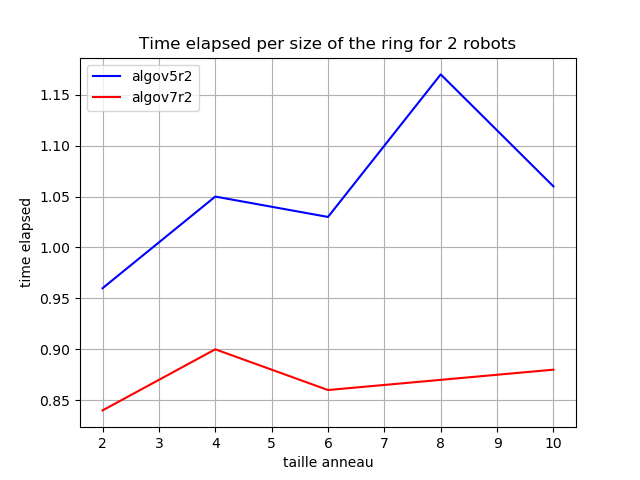
\includegraphics[width=0.5\textwidth]{../data/data-phiSimple/compar_phiSimple_2.png}\label{phiSimpler2}}
    \subfloat[][]{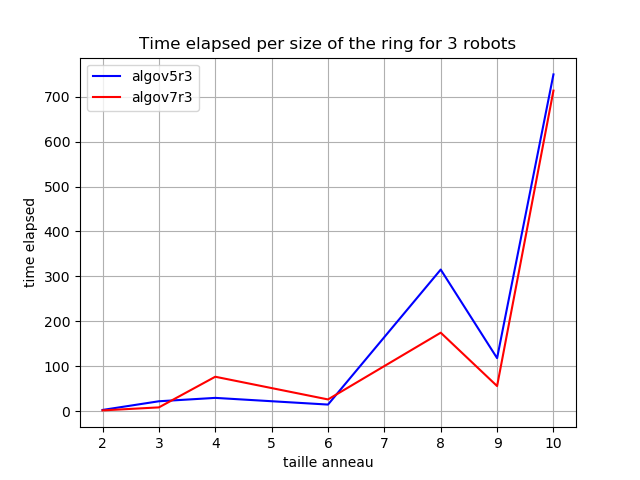
\includegraphics[width=0.5\textwidth]{../data/data-phiSimple/compar_phiSimple_3.png}\label{phiSimpler3}}
    \caption{Results for 2 (a) \& 3 (b) robots}
\end{figure}

\subsection{Test $\phi_{SM}$}

Now we test $\phi_{SM}$, a strategy a bit more elaborate that should be harder to solve and more relevant. Here, the timeout is 6h (21600s).

\begin{figure}[!h]
    \centering
    \subfloat[][]{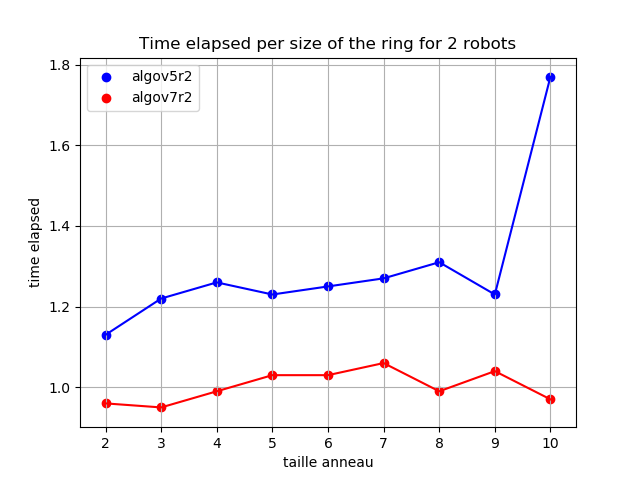
\includegraphics[width=0.5\textwidth]{../data/data-phiSM/compar_phiSM_2.png}\label{phiSMr2}}
    \subfloat[][]{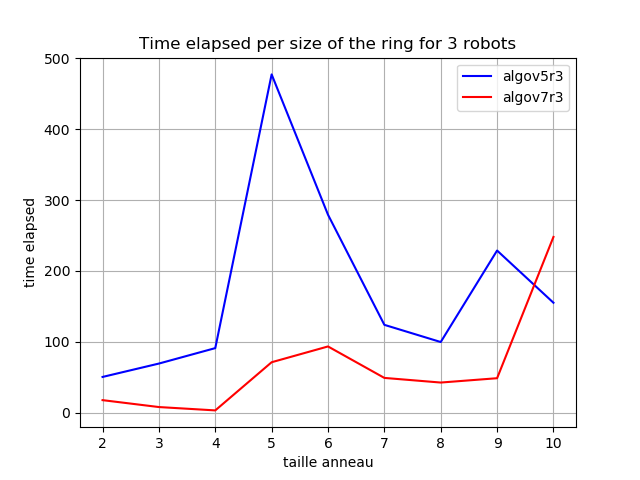
\includegraphics[width=0.5\textwidth]{../data/data-phiSM/compar_phiSM_3.png}\label{phiSMr3}}
    \caption{Results for 2 (a) \& 3 (b) robots}
\end{figure}

\begin{figure}[!h]
    \centering
    \subfloat[][]{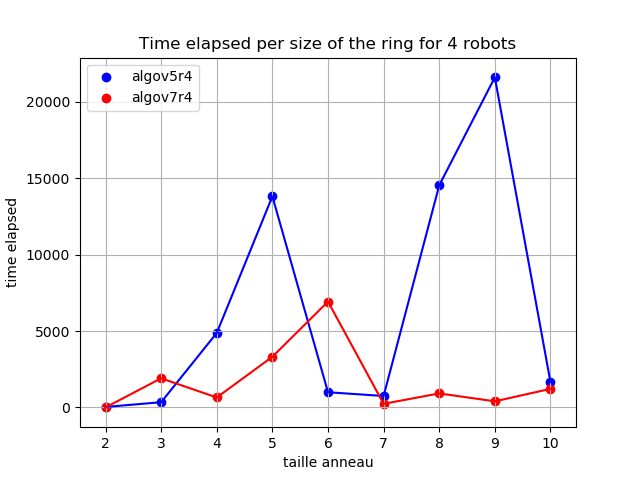
\includegraphics[width=0.5\textwidth]{../data/data-phiSM/compar_phiSM_4.png}\label{phiSMr4}}
    \subfloat[][]{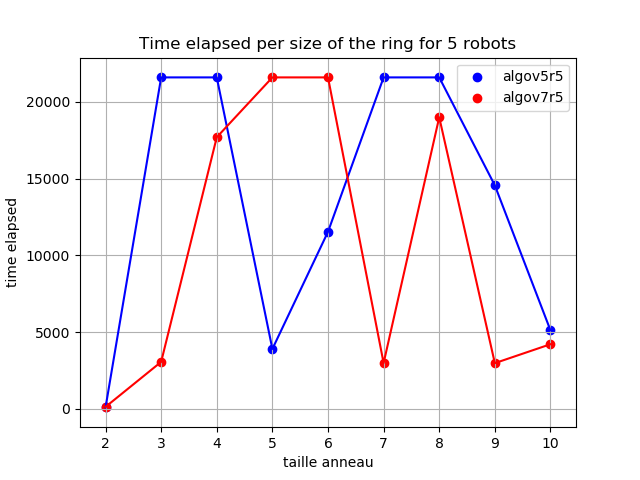
\includegraphics[width=0.5\textwidth]{../data/data-phiSM/compar_phiSM_5.png}\label{phiSMr5}}
    \caption{Results for 4 (a) \& 5 (b) robots}
\end{figure}

\subsection{Test $\phi_{R}$}

Finally, we test $\phi_{R}$ the most complex strategy that we have.

\begin{figure}[!h]
    \centering
    \subfloat[][]{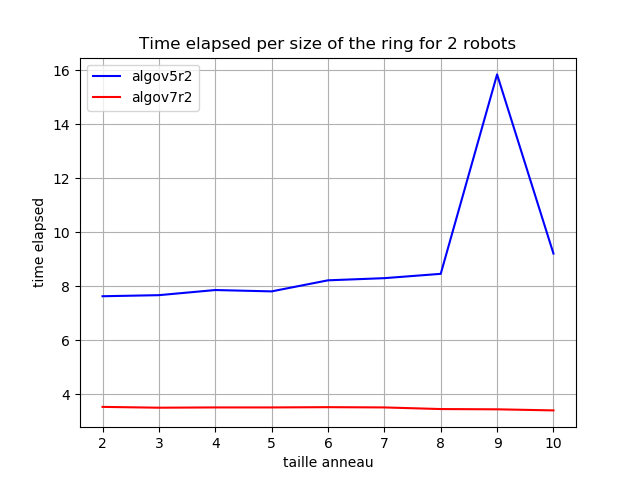
\includegraphics[width=0.5\textwidth]{../data/data-phiR24/compar_phiR24_2.png}\label{phiR24r2}}
    \subfloat[][]{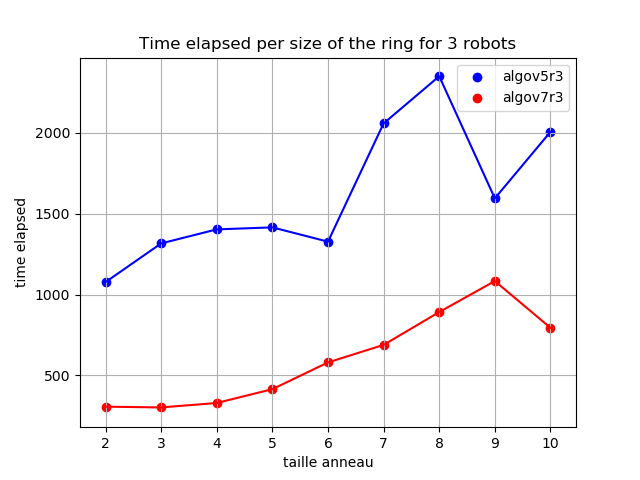
\includegraphics[width=0.5\textwidth]{../data/data-phiR24/compar_phiR24_3.png}\label{phiR24r3}}
    \caption{Results for 2 (a) \& 3 (b) robots}
\end{figure}

\begin{figure}[!h]
    \centering
    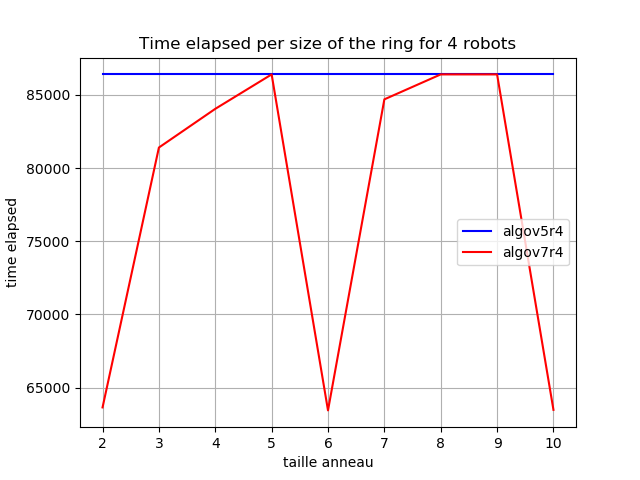
\includegraphics[width=0.6\textwidth]{../data/data-phiR24/compar_phiR24_4.png}\label{phiR24r4}
    \caption{Results for 4 robots}
\end{figure}
\newpage
\printbibliography %Prints bibliography
\end{document}